\section{Effective configurations and architectures}
\label{app:config}
Table~\ref{tab:full-config} records the settings that distinguish the three configurations. All nine effective JSON snapshots are provided in \path{evidence/runs/}. A paired S0/S1 run changes only the color-jitter switch in the model and training design. The frozen pilot reference and run name identify each execution.

\begin{table}[H]\centering\small
\caption{Effective experiment settings. Trainable counts exclude buffers.}\label{tab:full-config}
\begin{tabularx}{\linewidth}{@{}lYYY@{}}\toprule
Setting & U & S0 & S1 \\ \midrule
Architecture & Compact U-Net & SegFormer-B0 & SegFormer-B0 \\
Initialization & Scratch & ADE20K pretrained with new head & Same per-seed state as S0 \\
Trainable / frozen & 1,964,369 / 0 & 3,718,513 / 0 & 3,718,513 / 0 \\
Learning rate & $10^{-3}$ & $6\times10^{-5}$ & $6\times10^{-5}$ \\
Training color jitter & Off & Off & On with probability 0.5 \\
Output classes & 17 & 17 & 17 \\ \bottomrule
\end{tabularx}
\end{table}

The shared budget uses AdamW with weight decay 0.01, batch size 4, up to 40 epochs, patience 8, full 32-bit precision, no scheduler and disabled TF32. The target uses ignore 255 and the loss is CE plus soft Dice with weights 1 and 1. Source and preprocessing are checked against the fixed split manifest before a run. The loader uses zero workers in the recorded run protocol.

The U-Net encoder channels are 16, 32, 64, 128 and 256. Each double-convolution block uses $3\times3$ convolutions, GroupNorm with eight groups and ReLU. The upsampling path concatenates skip features and uses the same block type. The SegFormer encoder has four stages with widths 32, 64, 160 and 256, attention heads 1, 2, 5 and 8, and spatial-reduction ratios 8, 4, 2 and 1\cite{segformerconfig}. The decoder projects each stage to width 256 and uses an aligned fusion head.

\clearpage
\section{Per-seed results and run provenance}
\label{app:runs}
\begingroup
\setstretch{1.06}
\setlength{\intextsep}{7pt}
Table~\ref{tab:final-seed-results} reports the held-out scores. Table~\ref{tab:validation-best} reports validation metrics at the epochs selected for test.

\begin{table}[H]\centering\small
\caption{Selected validation checkpoints. The three overlap columns are percentages.}\label{tab:validation-best}
\begin{tabular}{@{}rlrrrrr@{}}\toprule
Seed & Run & Best epoch & FG mIoU & FG Dice & Trash mIoU & Loss \\ \midrule
69420 & U & 15 & 5.309 & 8.437 & 3.270 & 1.3902 \\
69420 & S0 & 15 & 19.534 & 28.051 & 13.787 & 1.1341 \\
69420 & S1 & 14 & 17.580 & 25.876 & 11.361 & 1.1386 \\
67 & U & 15 & 6.137 & 9.130 & 3.611 & 1.3118 \\
67 & S0 & 20 & 19.125 & 27.528 & 13.133 & 1.0426 \\
67 & S1 & 9 & 16.994 & 25.014 & 13.954 & 1.0869 \\
69 & U & 12 & 5.830 & 8.923 & 3.427 & 1.2957 \\
69 & S0 & 8 & 15.639 & 23.365 & 12.321 & 1.0800 \\
69 & S1 & 22 & 16.796 & 25.283 & 14.292 & 1.2067 \\
\bottomrule\end{tabular}

\end{table}

Table~\ref{tab:provenance} maps the score rows to their checkpoints. See \path{verified_results.json} for full IDs and hashes.
\begin{table}[H]\centering\small
\caption{Active run identifier and evaluated checkpoint fingerprint for each result.}\label{tab:provenance}
\begin{tabular}{@{}rllll@{}}\toprule
Seed & Run & Platform & Run ID prefix & Checkpoint SHA prefix \\ \midrule
69420 & U & Colab & \cls{59a5534d} & \cls{05aa0e8acf65} \\
69420 & S0 & Colab & \cls{44b2f727} & \cls{1dfcd83afce2} \\
69420 & S1 & Colab & \cls{9d2434a5} & \cls{5d6070706d75} \\
67 & U & Kaggle & \cls{520488aa} & \cls{cf6df95b2a78} \\
67 & S0 & Kaggle $\to$ Colab & \cls{73460d50} & \cls{aa669fc9ae93} \\
67 & S1 & Colab & \cls{5bbb6140} & \cls{08fbda83ed36} \\
69 & U & Colab & \cls{d11fd7e4} & \cls{aaf72e433d33} \\
69 & S0 & Colab & \cls{7c6af03c} & \cls{64f1f8cf41ed} \\
69 & S1 & Colab & \cls{c6cef0a6} & \cls{2c2868ab7113} \\
\bottomrule\end{tabular}

\end{table}

\begin{table}[H]\centering\small
\caption{S1 minus S0 validation deltas in percentage points and outcome of the proposal rule. The held-out deltas appear separately in Table~\ref{tab:final-paired-deltas}.}\label{tab:validation-deltas}
\begin{tabular}{@{}rrrrl@{}}\toprule
Seed & FG mIoU & FG Dice & Trash mIoU & Rule \\ \midrule
69420 & -1.953 & -2.175 & -2.425 & Not met \\
67 & -2.131 & -2.515 & +0.821 & Not met \\
69 & +1.157 & +1.917 & +1.971 & Met \\
\bottomrule\end{tabular}

\end{table}
\endgroup

\clearpage
\section{Additional class-level results}
\label{app:class}
The class means and sample standard deviations in Tables~\ref{tab:class-iou} and \ref{tab:class-dice} use the three repeated evaluations of the same 1,078 test images. Pixel support counts each test pixel once. All 17 classes have nonzero target support. The final column of Table~\ref{tab:class-iou} is the mean of the three paired seed differences in IoU.

\begin{table}[H]\centering\footnotesize
\caption{Held-out per-class IoU, mean $\pm$ sample SD (\%). S1--S0 is in percentage points.}\label{tab:class-iou}
\begin{tabular}{@{}rlrrrrr@{}}\toprule
ID & Class & Test pixels & U & S0 & S1 & S1--S0 (pp) \\ \midrule
0 & \cls{background} & 168,351,826 & $91.33\pm 0.32$ & $93.36\pm 0.15$ & $93.14\pm 0.10$ & -0.22 \\
1 & \cls{rov} & 7,661,326 & $41.00\pm 5.30$ & $52.82\pm 0.66$ & $52.06\pm 1.04$ & -0.77 \\
2 & \cls{plant} & 752,406 & $0.94\pm 0.58$ & $8.59\pm 3.89$ & $16.62\pm 14.49$ & +8.03 \\
3 & \cls{animal_fish} & 1,793,990 & $10.75\pm 6.14$ & $60.94\pm 14.22$ & $56.54\pm 1.50$ & -4.40 \\
4 & \cls{animal_starfish} & 25,521 & $0.13\pm 0.23$ & $0.04\pm 0.06$ & $0.18\pm 0.21$ & +0.14 \\
5 & \cls{animal_shells} & 6,789 & $0.72\pm 1.24$ & $2.44\pm 1.63$ & $3.76\pm 0.75$ & +1.32 \\
6 & \cls{animal_crab} & 223,331 & $0.97\pm 1.68$ & $46.26\pm 12.25$ & $41.97\pm 13.81$ & -4.30 \\
7 & \cls{animal_eel} & 87,276 & $3.02\pm 1.86$ & $29.55\pm 10.20$ & $27.76\pm 6.29$ & -1.80 \\
8 & \cls{animal_etc} & 201,098 & $0.43\pm 0.72$ & $0.26\pm 0.39$ & $0.71\pm 1.19$ & +0.44 \\
9 & \cls{trash_etc} & 1,822,549 & $4.72\pm 1.46$ & $11.34\pm 4.90$ & $8.00\pm 7.03$ & -3.34 \\
10 & \cls{trash_fabric} & 400,513 & $0.50\pm 0.83$ & $6.72\pm 5.81$ & $10.98\pm 0.75$ & +4.26 \\
11 & \cls{trash_fishing_gear} & 244,584 & $0.00\pm 0.00$ & $0.77\pm 0.35$ & $0.84\pm 1.46$ & +0.08 \\
12 & \cls{trash_metal} & 1,450,361 & $0.49\pm 0.54$ & $3.31\pm 1.04$ & $2.80\pm 0.81$ & -0.50 \\
13 & \cls{trash_paper} & 63,828 & $0.00\pm 0.00$ & $0.14\pm 0.24$ & $0.00\pm 0.00$ & -0.14 \\
14 & \cls{trash_plastic} & 2,822,298 & $8.53\pm 1.76$ & $19.72\pm 8.54$ & $13.85\pm 4.21$ & -5.87 \\
15 & \cls{trash_rubber} & 53,751 & $0.01\pm 0.02$ & $0.00\pm 0.00$ & $0.02\pm 0.04$ & +0.02 \\
16 & \cls{trash_wood} & 378,513 & $0.10\pm 0.17$ & $10.78\pm 5.84$ & $10.54\pm 2.75$ & -0.24 \\
\bottomrule\end{tabular}

\end{table}
Plastic has the largest IoU decline among trash classes in the paired means. Paper and rubber have low IoU across configurations, and have substantially fewer test pixels than plastic.

\begin{table}[H]\centering\footnotesize
\caption{Held-out per-class Dice, mean $\pm$ sample SD (\%).}\label{tab:class-dice}
\begin{tabular}{@{}rlrrrr@{}}\toprule
ID & Class & Test pixels & U & S0 & S1 \\ \midrule
0 & \cls{background} & 168,351,826 & $95.47\pm 0.17$ & $96.57\pm 0.08$ & $96.45\pm 0.06$ \\
1 & \cls{rov} & 7,661,326 & $58.02\pm 5.35$ & $69.13\pm 0.57$ & $68.46\pm 0.90$ \\
2 & \cls{plant} & 752,406 & $1.86\pm 1.15$ & $15.67\pm 6.55$ & $26.75\pm 21.27$ \\
3 & \cls{animal_fish} & 1,793,990 & $19.03\pm 10.36$ & $75.07\pm 11.14$ & $72.23\pm 1.23$ \\
4 & \cls{animal_starfish} & 25,521 & $0.27\pm 0.45$ & $0.08\pm 0.13$ & $0.35\pm 0.43$ \\
5 & \cls{animal_shells} & 6,789 & $1.40\pm 2.43$ & $4.74\pm 3.08$ & $7.25\pm 1.38$ \\
6 & \cls{animal_crab} & 223,331 & $1.89\pm 3.27$ & $62.65\pm 10.97$ & $58.26\pm 13.30$ \\
7 & \cls{animal_eel} & 87,276 & $5.82\pm 3.49$ & $45.00\pm 11.87$ & $43.20\pm 7.72$ \\
8 & \cls{animal_etc} & 201,098 & $0.85\pm 1.41$ & $0.53\pm 0.78$ & $1.39\pm 2.33$ \\
9 & \cls{trash_etc} & 1,822,549 & $8.99\pm 2.67$ & $20.14\pm 8.09$ & $14.31\pm 11.67$ \\
10 & \cls{trash_fabric} & 400,513 & $0.98\pm 1.63$ & $12.24\pm 10.08$ & $19.78\pm 1.22$ \\
11 & \cls{trash_fishing_gear} & 244,584 & $0.00\pm 0.00$ & $1.52\pm 0.70$ & $1.64\pm 2.84$ \\
12 & \cls{trash_metal} & 1,450,361 & $0.97\pm 1.07$ & $6.39\pm 1.97$ & $5.44\pm 1.54$ \\
13 & \cls{trash_paper} & 63,828 & $0.00\pm 0.00$ & $0.28\pm 0.48$ & $0.00\pm 0.00$ \\
14 & \cls{trash_plastic} & 2,822,298 & $15.69\pm 3.00$ & $32.38\pm 11.81$ & $24.17\pm 6.42$ \\
15 & \cls{trash_rubber} & 53,751 & $0.03\pm 0.04$ & $0.00\pm 0.00$ & $0.05\pm 0.08$ \\
16 & \cls{trash_wood} & 378,513 & $0.19\pm 0.33$ & $19.13\pm 9.29$ & $18.99\pm 4.44$ \\
\bottomrule\end{tabular}

\end{table}
Dice shows the same broad class-level difficulties. The bundled per-run confusion matrices retain the exact counts behind both measures.

\begin{table}[H]\centering\small
\caption{Percentage of true foreground or trash pixels assigned to background, by seed and model.}\label{tab:appendix-background}
\begin{tabular}{@{}rrrrrrr@{}}\toprule
Seed & U FG & S0 FG & S1 FG & U trash & S0 trash & S1 trash \\ \midrule
69420 & 51.00 & 34.43 & 33.24 & 62.50 & 57.43 & 60.25 \\
67 & 42.88 & 29.41 & 33.56 & 53.04 & 50.84 & 60.91 \\
69 & 43.77 & 30.01 & 35.22 & 53.12 & 50.01 & 58.31 \\
\bottomrule\end{tabular}

\end{table}
Every row shows a higher trash-to-background rate for S1 than for S0, despite the different directions of the trash mIoU changes. The CSV also provides the pixel numerators and denominators.

\clearpage
\section{Training histories for all nine runs}
\label{app:curves}
Figure~\ref{fig:all-curves} shows the saved epoch histories underlying the best-epoch and early-stopping results. Each row uses a common x-axis and each metric uses the same y-scale across seeds. Dots mark the epochs evaluated on test.
\begin{figure}[H]\centering
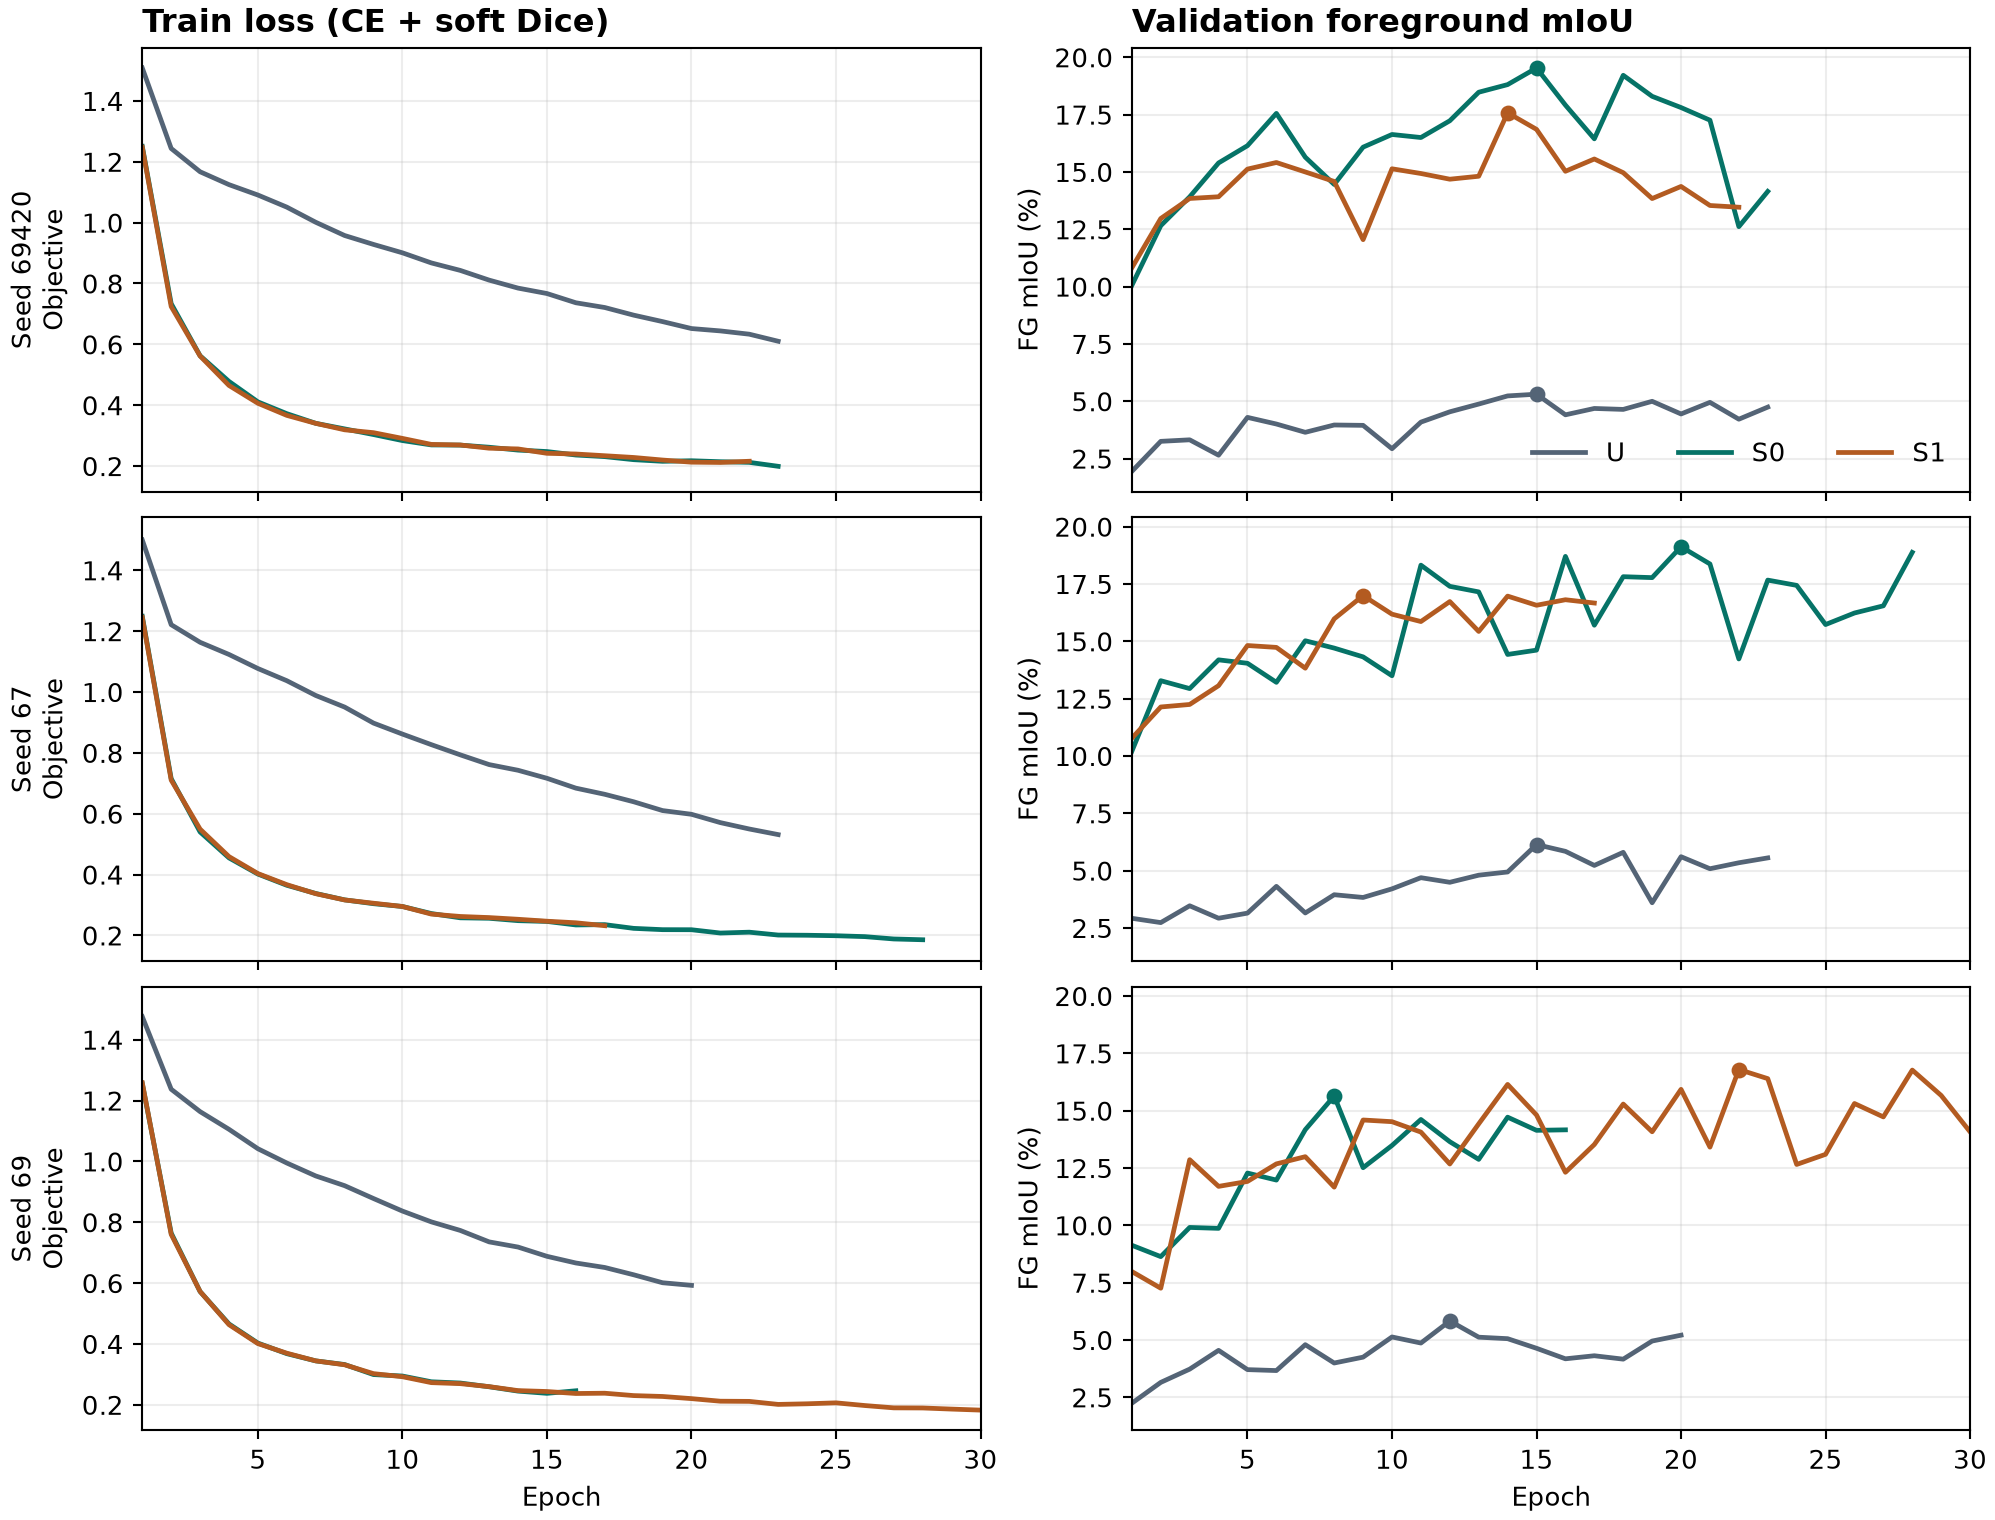
\includegraphics[width=\textwidth]{images/all_seed_curves.png}
\caption{Train objective and validation foreground mIoU for U, S0 and S1 across all seeds. Curves stop at the last completed epoch.}\label{fig:all-curves}
\end{figure}
Both SegFormer configurations reach higher validation foreground mIoU than U at every seed. The differing peak positions explain why early stopping runs for different numbers of epochs under the same patience.

\clearpage
\section{Verification and continuation notes}
\label{app:verify}
The source revision and common dataset identities are listed below. The archive SHA-256 hashes the raw ZIP bytes. The manifest digest hashes its canonical content. The test membership digest binds the ordered test rows.
\begin{description}
\item[Source revision] \path{7df323698d1ae4d5122850a54eb38b01609d80f1}
\item[Archive SHA-256] \path{caf93d992b85343cfc500386c94ca9ffa6c63e2284e04127753a40db8f33ba4c}
\item[Manifest content digest] \path{87905f1a97dd2c04194e049ca61d1a7f3bbe2942e9fe17dc2d737c371cdce943}
\item[Test membership digest] \path{738b95e533e0dc479c247f5a0c62d1298dec6a0d15cc65b88a71b689f1c7e147}
\end{description}

The 8 November audit checked export hashes, test/checkpoint and membership binding, history order, validation checkpoint selection and per-class metrics. The nine test outputs each contain 186,339,960 valid pixels after excluding ignore and padding. Raw test results come from the recorded GPU inference runs. The packaged verifier recomputes metrics from those saved counts.

Table~\ref{tab:continuation} records three execution paths that require care when reading the results.
\begin{table}[H]\centering\small
\caption{Continuation and replay evidence. Epochs count within the same experiment.}\label{tab:continuation}
\begin{tabularx}{\linewidth}{@{}lYY@{}}\toprule
Run & Recorded event & Evidence treatment \\ \midrule
S0, seed 67 & Resumed after epoch 7 from Kaggle on Colab and finished at epoch 28. & Retains the common history prefix and seed. Labeled as a mixed runtime. \\
U, seed 69 & Training ended at epoch 20. Replay of the epoch-12 validation checkpoint changed nine confusion cells. & Half the absolute count difference was five of 176,765,049 valid pixels. The narrow replay receipt is bound to the audited artifacts. Test evaluates the original best checkpoint. \\
S1, seed 69 & Continued after epochs 21 and 28. Finished at epoch 30 with best epoch 22. & Parent checkpoint hashes and history prefixes preserve one experiment across resumes. \\
\bottomrule\end{tabularx}
\end{table}
The retained validation replay receipt and available raw T4 timing logs are included under the relevant run folders. Model state and optimizer/RNG state are stored separately in the original checkpoint archives. Exact continuation depends on those archives and their numerical runtime settings.
